% !TEX root = ../Documentation.tex

\section{Analysis}
\label{sec:analysis}
In this section, we analyze the previous Ampersand parser in order to understand its workings and signal the improvement points.

\subsection{System overview (R-M)}
The requirements of the new parser have been described in the project planning \citenac{plan}.
Basically, both the old and the new parser must be able to make a conversion from a text file (ADL-script) to a parse tree (the P-structure).
\autoref{fig:data-flow-1} depicts this data flow.
%
\begin{figure}[htb!]
	\centering
	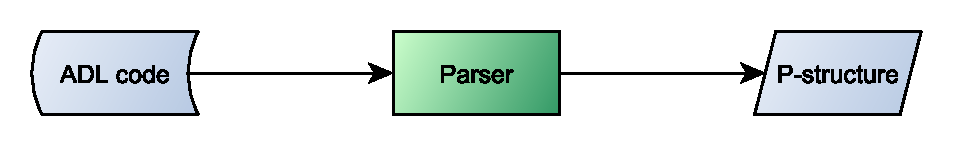
\includegraphics[width=0.586\textwidth]{Figures/DataFlow1}
	\caption{Relevant data flow for the Ampersand parsing component}
	\label{fig:data-flow-1}
\end{figure}

Often, the parsing component is separated into a lexer (that converts text to tokens) and the actual parser (that converts the tokens into the parse tree).
Since this separation is considered beneficial for both maintainability and performance \citeac{parsec}, we assumed from the beginning that the new Ampersand parser would be separated in this way.
This is depicted in \autoref{fig:data-flow-2}.
The previous parser also had a separate lexer, but the name was scanner instead.
%
\begin{figure}[htb!]
	\centering
	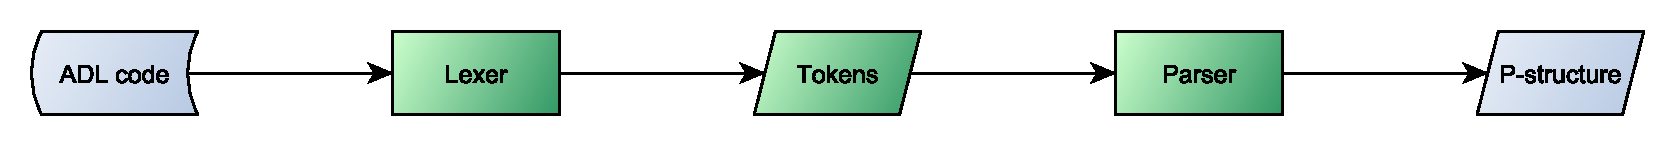
\includegraphics[width=1\textwidth]{Figures/DataFlow2}
	\caption{Data flow for the Ampersand lexing and parsing components}
	\label{fig:data-flow-2}
\end{figure}

In order to take the next steps and understand how the parser can be designed, we first take a look at the grammar in \autoref{subsec:analysis-grammar} and the parse tree in \autoref{subsec:analysis-parse-tree}.
Afterwards, we analyze the lexer with the original token structure, so that we can define a new token structure, in \autoref{subsec:analysis-lexer}.
Finally, we analyze the parser in \autoref{subsec:analysis-parser} and the generated errors in \autoref{subsec:analysis-errors}.

\subsection{Grammar (M)}
\label{subsec:analysis-grammar}
\dict{EBNF}{Extended Backus-Naur Form}%
\dict{Extended Backus-Naur Form}{Notation technique for documenting context-free grammars}%

\subsection{Getting the EBNF in good shape}
The Ampersand syntax is described using the EBNF notation. 
At the beginning of the project, we noticed that the existing EBNF diagram was not in line anymore with the actual syntax of Ampersand.
As the EBNF is a crucial source of information in building the new parser, the first focus was to update the old EBNF to represent the actual Ampersand Syntax.

Through reverse engineering, we checked all Haskell functions on the actual syntax they implement.
In the source of the new parser, all the syntax notations are placed above the actual parser function to support code maintainability.

The derived, and up to date, syntax is visualized using a railroad diagram, an ideal technique to visualize context free grammars.
Several railroad diagram generators are available on the internet, free of charge.
We used the railroad diagram generator created by Gunter Rademacher, available on http://bottlecaps.de/rr/ui.
During the actual generation, the generator failed on the Ampersand Syntax, more precisely on the statement: Exp4 ::= Exp5 (( ';' Exp5 )* | ('!' Exp5)*)
Convinced of the correctness of the EBNF statement, we contacted the owner of the tool, and he discovered a bug in his tool which he corrected promptly.

\subsection{The actual EBNF diagram}

TODO: Show/describe the EBNF (maybe actual EBNF as attachment).
TODO: Note that this EBNF was not available, but we had to derive it from the parser.
TODO: Note that we helped the railroad site to resolve a bug.

One interesting plus is that during the project we found a bug in the Railroad Diagram Generator.
The tool would crash with the \hyperref[fig:ebnf-Trm4]{\texttt{Trm4}} expressions.
This bug was reported to the author Gunther Rademacher, who promptly fixed the issue.

\subsection{Parse tree (R-M)}
\label{subsec:analysis-parse-tree}
The parse tree (also known as P-structure) is a data structure that very much resembles the EBNF description.
The root of the tree is the \texttt{P\_Context} structure, and every leaf of the tree has a field for the location where it was found in the ADL code (the \texttt{Origin} structure).
The tree is consistently defined with the record syntax and is well documented.

However, the constructions are not completely pure, since some transformations are necessary from the ADL to the P-structure.
This forces the parser to do more than only parsing.
Also, the order of the fields can be confusing; sometimes \texttt{Origin} is the first field and sometimes it is not.

During this project, small changes to the parse tree have been done.
These changes are described in \autoref{subsec:design-parse-tree}.

\subsection{Lexer (M)}
\label{subsec:analysis-lexer}
TODO: describe the possible improvements in the old lexer.

\subsubsection{Token structure}
TODO: Describe the old token strucure

\subsubsection{New token structure}
TODO: Develop a better token structure

\subsection{Parser (R-M)}
\label{subsec:analysis-parser}
The previous Ampersand parser was generally well organized, so each ENBF rule could be mapped to a different parser.
However, several flaws were observed as improvement points.
During this project, we focused on the following issues:
\begin{description}
  \item[Lacking documentation]
    There was no documentation on the recognized grammar.
    The last EBNF available was not updated in a long while.
  
  \item[Ad-hoc transformations]
    The parser was built with the applicative interface of the uulib.
    The applicative operators were thus used in sequence to recognize each of the accepted grammar productions.
    However, the parser was often forced to change the order and format of the parsed structures, because the parse tree did not match the grammar productions (i.e. many rebuild functions).
    
  \item[Long file]
    Since all the grammar constructions -- plus help functions -- were in a single file, the parser was hardly readable.
    It summed a total of 823 lines of code only in the \texttt{Parser} module.
  
  \item[Pretty printing]
    It used to be impossible to print the parse tree back to ADL-code.
    That made it harder to develop and test the parser properly.
  
  \item[Test suite]
    There were no automated tests for the parser.
    Because of this, any code change would be hard to test and could potentially influence other Ampersand modules.
  
  \item[Duplicated code]
    A large part of the code was duplicated and not used (mainly in the \texttt{Parsing} module).
  
  \item[Error messages]
    As mentioned, the main reason for this project was the bad quality of the error messages generated.
    \autoref{subsec:analysis-errors} expands on this point.
\end{description}
%
Although it may be hard to resolve all the mentioned issues, we believe our efforts have played off well.
In \autoref{subsec:design-parser} we describe how the new parser was designed.

\subsection{Errors (M)}
\label{subsec:analysis-errors}
TODO: show how the parser did not provide good errors, and how we could improve them.
